\documentclass[12pt]{report}
\pagestyle{headings}
\usepackage{rotating}
\usepackage{graphicx}
\usepackage{longtable}
\usepackage[tt]{titlepic}
\usepackage{verbatim}
\setlength{\parindent}{0.0in}
\setlength{\parskip}{0.1in}
\setcounter{secnumdepth}{1}
\setcounter{tocdepth}{1}

\addtolength{\textheight}{2cm}
%\addtolength{\footskip}{2cm}

\newcommand\placeholder[2]{
	\noindent
	{\setlength{\fboxsep}{0pt}
		\makebox[#1]{
			\parbox{0pt}{\rule{0pt}{#2}}
			\parbox{#1}{\centering
				
\includegraphics[width=0.50\textwidth]{logo.ps}
			}
		}
	}
}

\author{Holger Ludvigsen,\\Vegar Neshaug,\\Jon Skarpetveit,\\Rahele Zarabi,\\Christoffer Etellerannet}
\title{{\small Eksperter i Team\\TPG4850 VR-Landsbyen}\\\textbf{Team 4 (V.I)}}
\date{{\small \today}}
\titlepic{\placeholder{\textwidth}{0.5\textwidth}}

\begin{document}
\maketitle

\pagenumbering{roman}

\begin{verbatim}

\chapter*{Summary of report}
	As a part of the course Experts in Team (EiT) at NTNU, five students were put in a group to collaborate on a project. This team (us) was a part of the virtual reality village of EiT, and came up with the following problem statement:

\begin{center}\em How can you make an affordable and usable prototype\\for head tracking to be used for virtual reality?\end{center}
\vspace{\parskip}

We solved this problem by first doing a preliminary study followed by design and imlementation of the solution. In the preliminary study, several technical and theoretical subjects were investigated. The mathematics behind estimation of object position from pictures were elaborated. We looked at the available technology for connecting a high definition camera to a PC and reading the images from it. We studied the properties of infrared light. We checked out and tested the Nintendo Wii and its Wiimotes. Lastly, potential areas of use for a solution was described.

Then, a specification of the requirements was carefully crafted. The specification was the basis for the design of the solution. This design specifies how the components of the system is constructed and how they are connected. The components of the system make up a pipeline:

\begin{figure}[h]
\centering
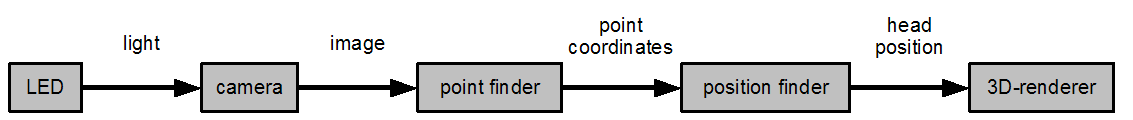
\includegraphics[width=\textwidth]{graphics/main_design_english.png}
\end{figure}

The LED-component is a set of infra red LEDs that are attached to the user's head. These transmit light that is captured by a high definition camera. The image from this camera is read by a point finder software that attempts to locate the coordinates of the bright dots in the image where the LEDs are. These coordinates are transferred to the position finder software which uses them to estimate the position of the user's head. This head position is then used by the 3D-renderer software to display a 3D-scene on a screen where the viewpoint is mapped to the head position.

Course
Project group
Problem statement
Prestudy
How solved:
	Reqspec
	Design
	Implementation
Result
Evaluation
Conclusion
	\pagebreak
	
\setlength{\parskip}{0.0in}
\tableofcontents
\listoftables
\listoffigures
\chapter*{Akronymliste}
\pagebreak
\setlength{\parskip}{0.1in}

\pagenumbering{arabic}
\setcounter{page}{1} % start normal page counting here

\chapter*{Introduksjon}

\part{Project plan}

	\input{project_plan_introduction.tex}
	
	\input{organization.tex}
	
	\input{project_context.tex}
	
		\input{risk_text.tex}
		
	\input{time_plan.tex}
	
	\input{project_plan_summary.tex}
	
\part{Preliminary Study}

	\input{pre_study_introduction.tex}
	
	\input{pre_study.tex}
	
	\input{pre_study_summary.tex}
	
\part{Requirement Engineering}

	\input{req_eng_introduction.tex}

	\input{req_eng.tex}
	
	\input{req_eng_summary.tex}
	
\part{Testing}

	\input{testing_introduction.tex}

	\input{testing.tex}
	
	\input{testing_summary.tex}
	
\part{Aftermath}

	\input{aftermath_introduction.tex}
		
	\chapter{The results}
		
	\chapter{Further work}
	
	\chapter{Evaluation}
	
	\input{aftermath_summary.tex}

\appendix

	

\pagestyle{plain}
\pagebreak
\pagenumbering{roman}
\setcounter{page}{1} % end normal page counting here

\begin{description}
	\item[1080i/p] At et kameras bilde har 1080 bildepunkter i h�yden og er interlaced/progressive (se interlacing og progressive)
	\item[3-dimensjonal] Se tre-dimensjonal
	\item[3D] Se tre-dimensjonal
	\item[3D-viseren] Delen av systemet som viser en 3D-scene p� skjermen
	\item[Akselerasjonsmeter] Sensor som m�ler akselerasjon
	\item[Bibliotek] Samling av kode som tilbyr nyttig funksjonalitet
	\item[Bluetooth] Type tr�dl�st nettverk
	\item[C] Et programmeringsspr�k
	\item[CCD-bildebrikke] En type brikke som kan fange et bilde til digital form
	\item[CMOS-bildebrikke] En type brikke som kan fange et bilde til digital form
	\item[Deinterlacing] � fjerne interlacing fra et bilde (se interlacing)
	\item[Diode] En type elektrisk lampe
	\item[DirectShow] Et bibliotek for � h�ndtere multimedia p� PC-er
	\item[HDMI] Et type grensesnitt for � sende digital lyd og bilde
	\item[Headsettet] Anretningen en bruker m� ha p� hodet for � bruke systemet
	\item[Intensitet] Lysstyrken til et bildepunkt
	\item[Intensity] Et stykke maskinvare for � gi HDMI-kontant til en PC
	\item[Interlacing] � sende annenhver linje av et bilde om gangen for � oppn� bedre filmkvalitet
	\item[Java] Et programmeringsspr�k
	\item[LED] Light emitting diode (se diode)
	\item[Lyspunkt] Omr�det i et bilde med h�y intensitet, sannsynligvis for�rsaket av at en lyskilde filmes
	\item[OpenGL] Et bibliotek for � vise 3D-grafikk p� PC-er
	\item[Oppl�sning] Antall bildepunkter i et bilde
	\item[PCI-express] En type tilkoblingpunkt i en PC
	\item[Piksel] Et bildepunkt
	\item[Posisjonsfinneren] Delen av systemet som finner posisjonen av hodet til brukeren
	\item[Progressive] Det motsatte av interlacing, dvs at alle linjene i et bilde sendes om gangen
	\item[Punktfinneren] Delen av systemet som finner koordinatene til lyspunktene i kamerabildene
	\item[StatoilHydro] Sponsor av VR-landsbyen
	\item[VR] Se virtual reality
	\item[Virtual reality] Simulering av virkelighet
	\item[Wii] Spillkonsoll fra Nintendo
	\item[Wiimote] Styrekontrolleren til Wii (se Wii)
\end{description}



\nocite {a1,a2,a3,a4,a5,a6,a7,a8,a9,a10,a11,a12,a13,a14,a15,a16,a17,a18,a19,a20,a21}
\bibliographystyle{plain}	
\bibliography{literature}
	
\end{verbatim}

\end{document}
